\documentclass[11pt]{article}
\usepackage{deauthor}
\usepackage{times}
\usepackage{graphicx}
\usepackage{hyperref}
\usepackage{wrap fig}
\usepackage{subcaption}

\begin{document}
\title{A Systematic View of Data Science}
\author{M. Tamer \"{O}zsu\\University of Waterloo\\tamer.ozsu@uwaterloo.ca}
%\maketitle

\section{Introduction}
In the June 2020 issue of this Bulletin, Jeffrey Ullman of Stanford University published an opinion piece that discussed the conflicting ownership claims of the field of ``data science'' by different communities, and made the case that the database community has a central role to play ~\cite{Ullman:2020aa}. I certainly subscribe to the points made by Jeffrey. When I was asked to write this article, I decided to take a more systematic view of data science. This is important for a number of reasons. First and foremost, it has been asked: is data science a discipline? This cannot be answered without a comprehensive and systematic analysis of what ``it'' is. My personal short answer is ``not yet'', but fully answering this question requires another article altogether. Certainly, there is progress in establishing data science as a discipline: academic programs and units are being formed, and academic publications are becoming established.  However, we need to investigate this area further to be able to define the ``core'' of data science in order for it to become its own discipline. There has been progress on these fronts, but I do not believe that we are there yet. 
 
The question of ``who is a data scientist?'' requires further clarification. The second reason for a comprehensive and systematic approach to the subject is my belief that data science is broad in scope, and involves far more areas than what we may typically think of. It is important to also include these areas in the discussion. Developing a robust answer to this question is not possible by being reactive; a holistic definition must include how different pieces fit and interact. 

Third, a systematic investigation of the field is likely to identify important issues that many of us may consider should be in the toolbox of a professional data scientist -- what might be called the ``core''. At a recent Data Science Leaders  (which has since been renamed Academic Data Science Alliance) annual meeting, a colleague opined that no one should try to form a data science institute or centre without first defining what ``data science'' means in the context of that organization. I strongly agree with that sentiment, so this is my attempt.

My objective in this article is to share my personal views on how we should be thinking about data science. Every one of us approach the field with our own academic backgrounds and perspectives, and our views are shaped by our biases and experiences. That is certainly true in my case. I led a proposal for a nation-wide data science centre in Canada a few years ago, and although that effort was not successful, I interacted with colleagues from different organizations and disciplines that forced me think carefully about how I view the field and how such an institute needs to be framed. I am currently leading an effort to map that vision to a data science institute at the University of Waterloo, which has furthered the evolution of my thinking. This article is based on the proposals written in collaboration with many colleagues as part of these efforts.

\section{What is Data Science?}

\emph{Data Science} is the term commonly used for the data-driven approach to solving problems, and involves the analysis of large volumes of data, extracting knowledge and insight from it, and using information for better decision-making. However, this is too vague to be useful as a working definition. Therefore, we must look further.

Wikipedia gives the following definition: ``data science, also known as data-driven science, is an interdisciplinary field of scientific methods, processes, algorithms, and systems to extract knowledge or insights from data in various forms, either structured or unstructured, similar to data mining''. This definition captures a number of important aspects: that it is an interdisciplinary field and that it involves extracting knowledge from multi-modal structured or unstructured data. However, it then goes on to say ``similar to data mining''. Leaving aside the fact that ``similar'' is an entirely unhelpful phrase in this context, roughly equating data science to data mining is very limiting.

%\begin{wrapfigure}{l}{0.15\textwidth}
%\includegraphics[width=0.9\linewidth]{letters/Figures/Hayashi.png}
%\caption{Earliest Mention of Term}
%\label{fig:hayashi}
%\end{wrapfigure}

The earliest use of the term ``data science'' that I could find is in a 1998 paper by Chikio Hayashi. His definition states: ``data science intends to analyze and understand actual phenomena with `data'. In other words, the aim of data science is to reveal the features or hidden structure of complicated natural, human, and social phenomena with data from a different point of view from the established or traditional theory and method'' \cite{Hayashi:1998aa}. This is a definition from the perspective of a statistician, and it is interesting in its contrast of data science with ``traditional [statistical] theory and method''. The roots of what we now consider as a fundamental characteristic of data science, namely that data and its analysis are at the core of understanding actual phenomena, is clearly stated.

%\begin{wrapfigure}{r}{0.15\textwidth}
%\includegraphics[width=0.9\linewidth]{letters/Figures/fourth.png}
%\caption{Earliest Mention of Term}
%\label{fig:hayashi}
%\end{wrapfigure}
I am sure that many members of this community are familiar with Jim Gray's work on data-intensive discovery, which is well-captured in the book by Hey et al. ~\cite{hey2009the}. To quote one passage: ``\ldots all sciences [are] moving from observational, to theoretical, to computational, and now to the Fourth Paradigm – Data-Intensive Scientific Discovery''. Gray concentrated his work on astronomy and demonstrated many techniques and methods that are useful to data science. A passage in the Foreword by Gordon Bell is interesting: ``We are at a stage of development that is analogous to when the printing press was invented. [\ldots] Using computers to gain understanding from data created and stored in our electronic data stores will likely take decades -- or less.'' Gordon wrote this over a decade ago, and in the intervening period, we have made many advances, but we are still in the early stages of development of the data science field.

\begin{figure}
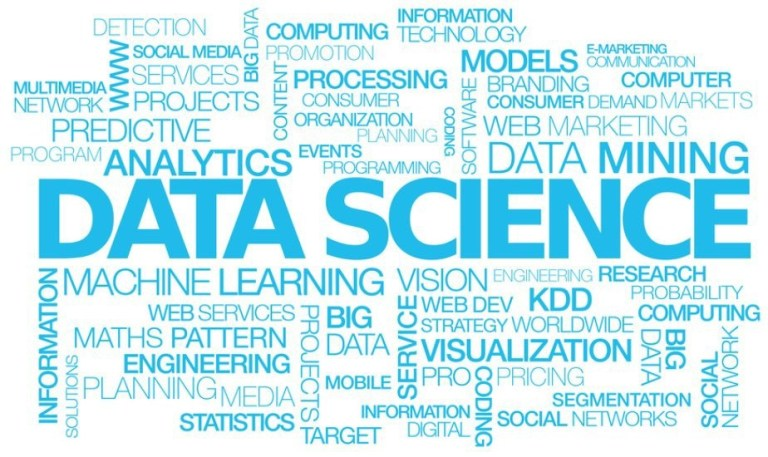
\includegraphics[width=0.9\linewidth]{letters/Figures/data-science-wordcloud.jpeg}
\caption{Data Science Word Cloud.}
\label{fig:dscloud}
\end{figure}

Each of these definitions captures some aspect of data science as a field, but a comprehensive and definitive identification of the field is still not available. A word cloud generated by Data Scientist\footnote{\url{https://thedatascientist.com/best-way-learn-data-science/}} indicates the diversity of viewpoints, or what some might call confusion, about the field (Figure~\ref{fig:dscloud}).


To me, a working definition that captures the essence of data science as a field is that \textit{data science is a data-driven approach to problem solving and scientific exploration that involves the process of collecting, managing, analyzing, explaining, and visualizing data and analysis results}. This definition captures both the breadth of the field and the areas where we need to develop depth. It provides a blueprint for developing research and teaching programs. This is the definition that shapes my perspective of the field.



\section{Drivers of Data Science}

There is a data-driven revolution underway in science and society, disrupting every form of enterprise. We are collecting and storing data more rapidly than ever before. However, our ability to leverage and use this data has been limited by the lack of knowledge exchange between experts in the sub-fields of data science, and by the lack of tools, methods, and principles for understanding and translating these insights into products, systems, and policies. McKinsey Global Institute estimates that the field of data science is currently generating \$1.3 trillion in economic value every year in the US; other countries have reported proportionally similar contributions. Although somewhat dated, a 2015 Organisation for Economic Co-operation and Development (OECD) report identified ``data-driven innovation'' (DDI) as having a central driving role in twenty-first century economies, defining DDI as ``the \textbf{use of data and analytics} to improve and foster new products, processes, organisational methods and markets'' \footnote{Emphasis from original OECD quote.}.

Canada has released a federal digital charter\footnote{\url{https://www.ic.gc.ca/eic/site/062.nsf/eng/h_00108.html}} that addresses the importance of data in the Canadian economy and establishes a vision for a data economy built around ten principles\footnote{These principles are: (1) Universal Access; (2) Safety and Security; (3) Control and Consent; (4) Transparency, Portability, and Interoperability; (5) Open and Modern Digital Government; (6) A Level Playing Field; (7) Data and Digital for Good; (8) Strong Democracy; (9) Free from Hate and Violent Extremism; and (10) Strong Enforcement and Real Accountability.}. The importance of this charter is in its multidisciplinarity and the need for engagement by a number of academic disciplines. The Information and Communications Technology Council of Canada has taken this charter and expanded it to involve provinces and municipalities, providing another dimension to complement the ten principles. It appears to me that, with proper positioning and attention, there is substantial potential for research within this framework.

Currently, the COVID-19 pandemic has clarified and emphasized the importance of data-based and data-driven decision-making. This topic deserves its own attention, and some day someone should write a good essay on data science approaches to pandemic management. Individual countries have differed in how well they have gathered, analyzed, and used data to make decisions; but globally, in my view, we have not done well, and this should be a major research agenda for the data science field.


\section{Data Science Ecosystem}

Data science is inherently multidisciplinary: it builds on a core set of capabilities in data engineering, analytics, security and privacy, as well as ethics (Figure \ref{fig:building}). Some of this core is technical, other components are not. The core exists in close interaction with application domains that leverage these capabilities to solve their most pressing problems. 

\begin{figure}[h]
\centering
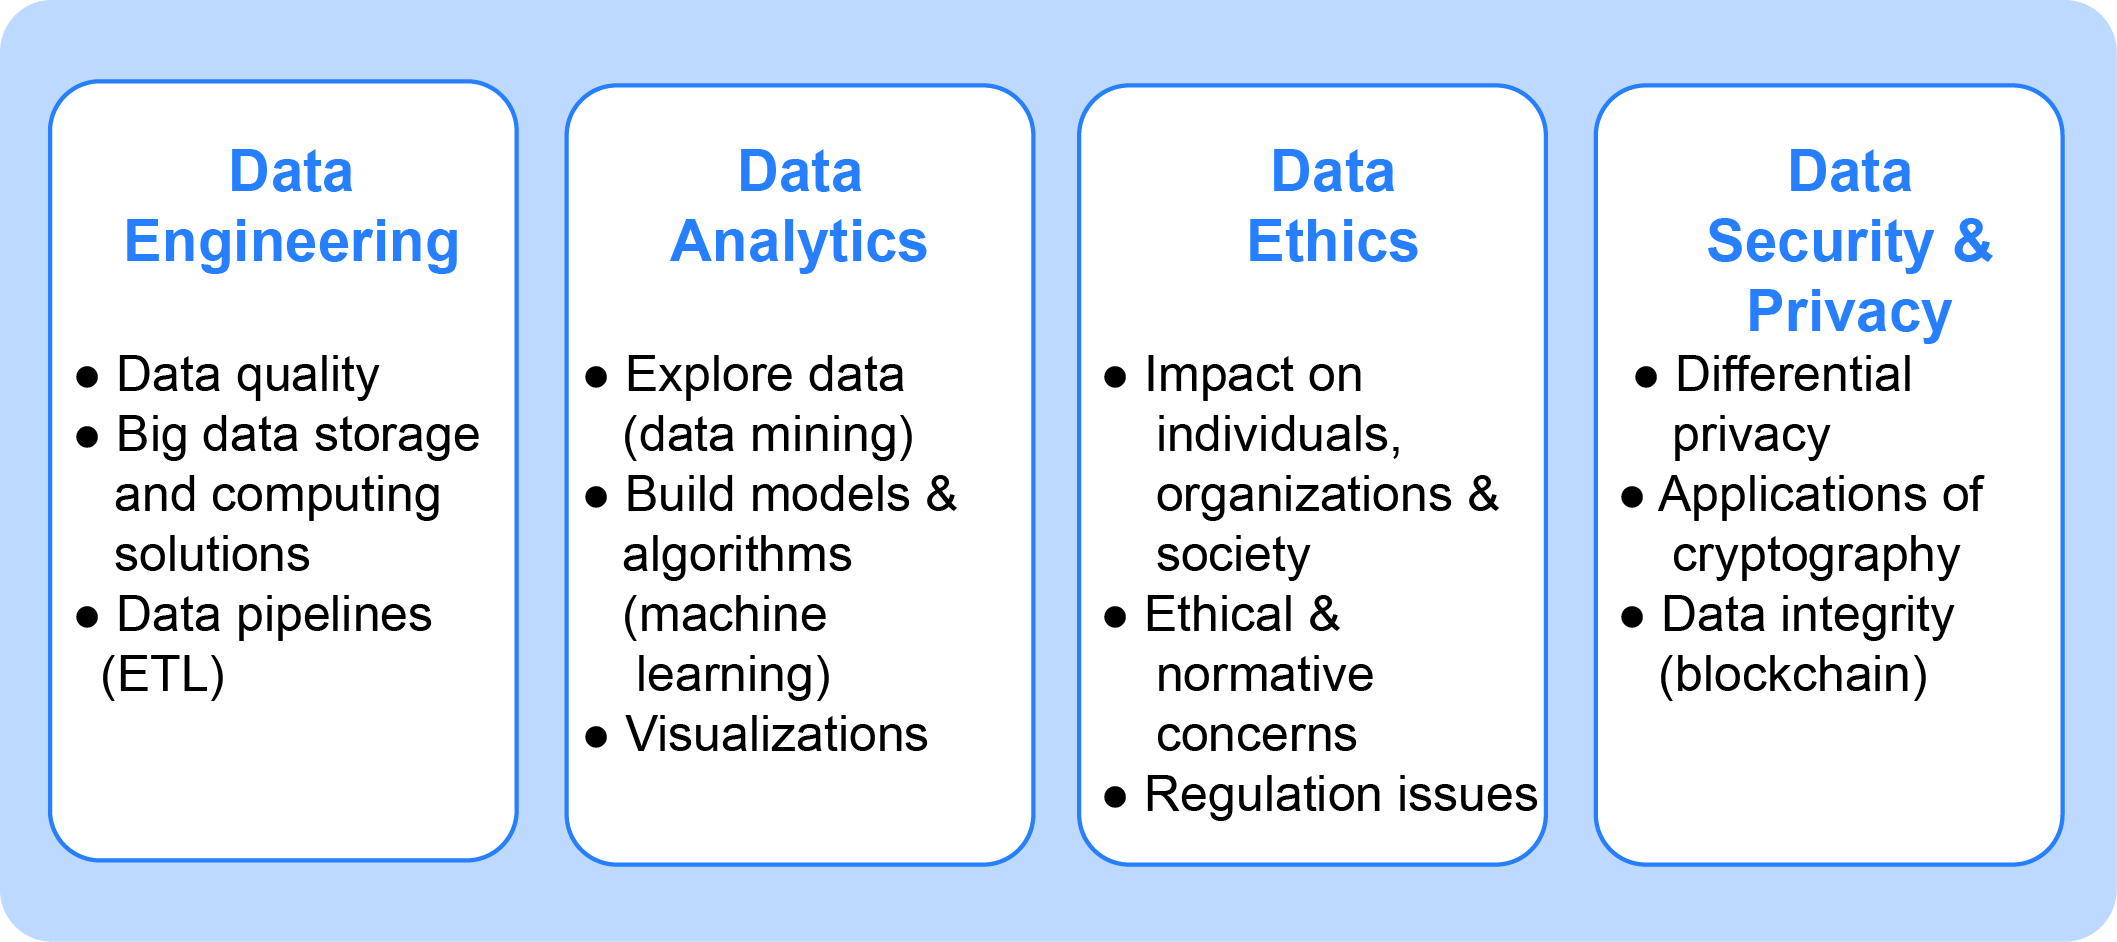
\includegraphics[scale=0.15]{letters/Figures/BuildingBlocks.jpg}
\caption{Data Science Building Blocks.}
\label{fig:building}
\end{figure}

An important aspect of data science is that it is application-driven. I do not mean to suggest that there is no application-independent core; what I am suggesting is that ultimately, data science seeks to solve a problem within an application area. This might be a ``problem'' in a domain (e.g., pandemic management in the age of COVID-19), or it may be ``exploration'' in an application domain (e.g., astrophysics), or it could be both (e.g., climate change). If we ignore the applications, we are in danger of only focusing on ``big data infrastructure'' issues. This would be a mistake, because we would be focusing only on the technology where we feel more comfortable, without leveraging the full force of data science. Therefore, the field requires the active involvement of domain experts from their respective application areas – without this combination of core technologies and application domains, it is difficult to talk about data science. In this sense, data science is a unifying field, requiring the participation of many disciplines and researchers (Figure \ref{fig:unify}).

\begin{figure}[h]
	\centering
	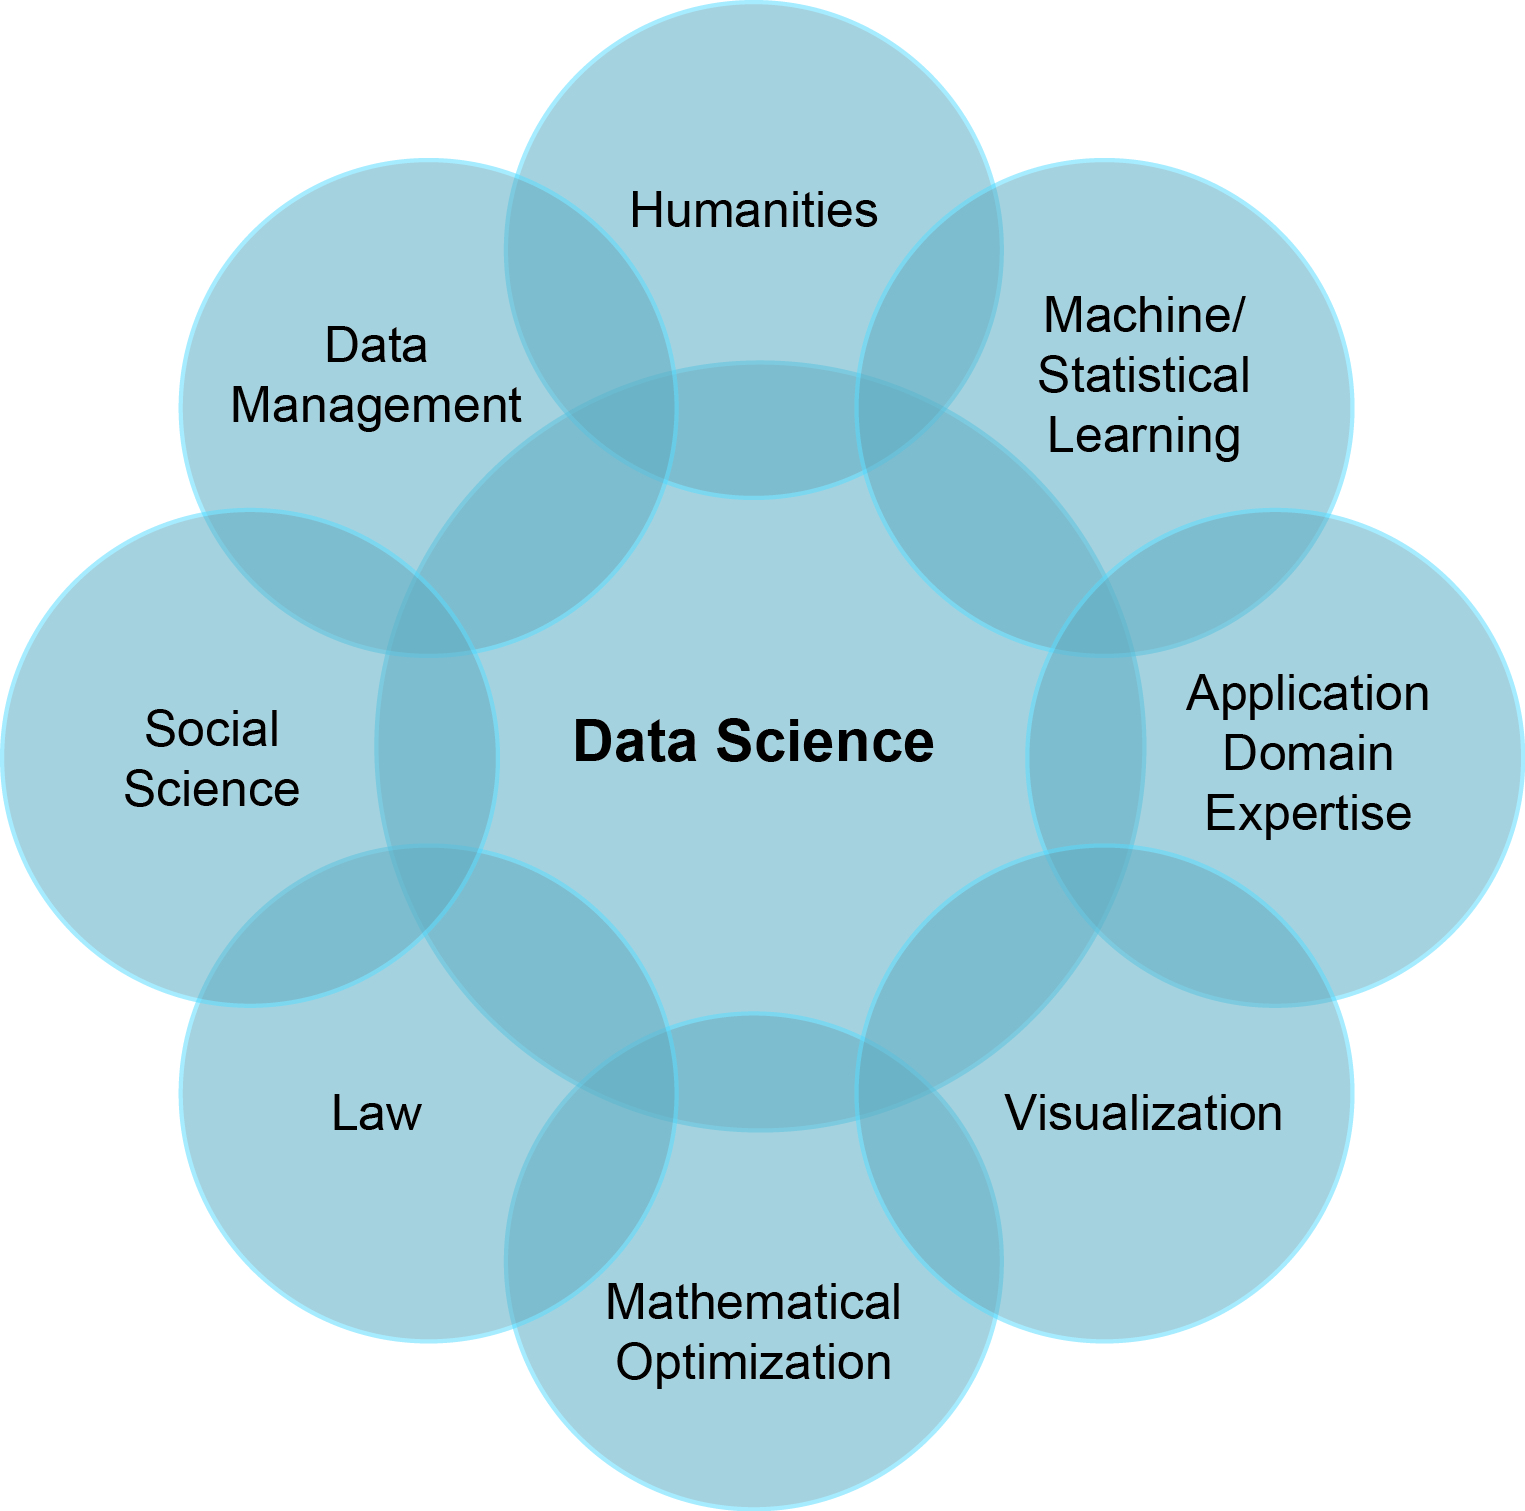
\includegraphics[scale=0.125]{letters/Figures/Unification.jpg}
	\caption{Data Science as a Unifier.}
	\label{fig:unify}
\end{figure}

These types of Venn diagrams are popular and have been produced by multiple communities. Jeff Ullman highlights how the statisticians view the field in terms of overlapping areas and gives his recommended revisions ~\cite{Ullman:2020aa}. Comparing these figures, my proposed diagram provides a more holistic and inclusive view of data science. 

Within this context, it is possible to think about the data science ecosystem in different ways. One way that I find useful is to think about it as a lifecycle: how data moves from collection and preparation to final decision-making. Another way to think about it is in terms of the software stack (or software infrastructure). As computer scientists, we usually end up thinking about things in terms of the software stack, which provides a different, but useful, viewpoint. I will consider both viewpoints in this section.

\subsection{Data Science Lifecycle}\label{sec:lifecycle}

 The ability to extract insight from massive datasets depends on a comprehensive, systematic, and end-to-end study of the data science lifecycle, as depicted in Figure \ref{fig:lifecycle}. The core consists of four technology stages that follow data through various processing steps, and two cross-cutting concerns. Data science applications leverage this core, and also inform meaningful technology development. I will summarize the scope of each element of the lifecycle and highlight its importance.

\begin{figure}[h]
	\centering
	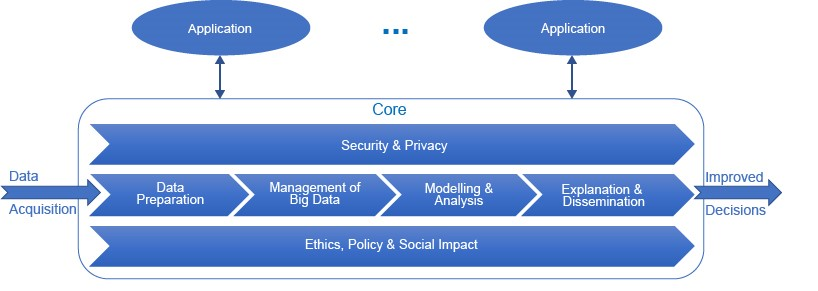
\includegraphics[scale=0.5]{letters/Figures/Lifecycle}
	\caption{Data Science Ecosystem.}
	\label{fig:lifecycle}
\end{figure}

\paragraph{Data Preparation.} Data science is based on data, and large volumes of data are collected from a variety of sources. Applying appropriate analysis to this data is a fundamental activity of data science; this is how new insights are obtained that can improve organizational effectiveness and efficiency, and result in evidence-informed decision-making. However, data must be adequate and relevant for the intended goal. Therefore, there is a need for methods for assessing the trustworthiness, reliability, validity, and fitness for use of large datasets. This stage focuses on challenges in data cleaning, data sampling, and the tracking of data provenance.

\paragraph{Management of Big Data.} I am going to say the least about this stage, since it is obvious to our community. The ``big data problem'' is something we have been working on for some time and the challenges are well-understood. Briefly, this stage of the workflow involves the development of a data management platform that provides appropriate functionality and interfaces for the execution of powerful, declarative queries for online exploration and large-scale data analysis.

\paragraph{Modelling and Analysis.} Modelling and analysis enable the derivation of insights from the data under study. In modern research in this area, the lines between statistics and computer science have become blurred. This blurring of lines is reflective of a ``best of both worlds'' approach, and there is an increasing realization that combining statistics and computer science leads to more effective analytics than relying on either field in isolation. Statistical reasoning brings a modelling framework that can be useful in interpreting results and expressing uncertainty, whereas machine learning techniques born out of computer science are often much better suited for making predictions from large datasets.

\paragraph{Explanation, Dissemination, and Retention.} An essential component of data science is ensuring that both data and analysis results are readily accessible to, and understandable by, all interested parties. These could include researchers, policy directors, industry leaders, and the public. It is important to develop new open-data platforms and data visualization techniques that will better enable users to understand data and to explore it with ease. Particular areas of investigation include data accessibility, visualization, lifecycle and retention, and interpretability.

\paragraph{Data Security and Privacy.} Data security and privacy are required from the time of data acquisition to the dissemination of results, as well as for secure archiving or deletion. An implicit goal of data science is to gain access to as much data as possible, which directly conflicts with the fundamental least-privilege security principle of providing access to the minimal resources necessary. Closing this gap includes careful re-design and advancement of security technologies to preserve the integrity of scientific results, data privacy, and to comply with regulations and agreements governing data access. This requires close collaboration with lifecycle technologies, with special attention to the particular needs of application domains.

\paragraph{Ethics, Policy, and Societal Impact.} Similar to data security and privacy, this is a cross-cutting aspect of data science that influences all other elements of the lifecycle. Let me briefly consider the three aspects of this element. Ethics of data use involves concerns related to data privacy and ownership, appropriate manipulation of data (what we can and cannot do to data), and fairness of algorithms. Data science never occurs in a vacuum -- there is always a policy context that influences what is possible, including the development of core technologies. The dual of this is that, hopefully, data science investigations will inform the development of meaningful public policy. It is equally important to always consider the impact of data science on: (1) individuals, (2) organizations, and (3) society as a whole.

\paragraph{Interactions Among Lifecycle Stages.} A disadvantage of any lifecycle definition is that it gives the impression that the entire process is linear and unidirectional. This is certainly not what I am arguing. The stages that comprise the technical core of data science are essential for creating these platforms. However, insular developments along these themes are not sufficient. It is essential to treat the lifecycle in a holistic manner to provide significant improvements in the end-to-end workflow for developing effective and efficient data science solutions. Some of these include issues at the intersections of stages, including data preparation and cleaning, the robustness of data analytics solutions and data contamination, data provenance management, better integration of data management and analysis, as well as data visualization and visual analytics.

\subsection{Software Infrastructure}

As I noted above, computer scientists like to think in terms of software architecture. In the data science context, this means ``big data infrastructure''. There are a number of ways this can be considered; I will reiterate what is described in our book \cite{OzsuV:2020aa} (Figure \ref{fig:bigdata}). Big data management relies on a distributed storage layer, whereby data is typically stored in files or objects distributed over the nodes of a shared-nothing cluster. Data stored in distributed files are accessed directly by a data processing framework that enables programmers to express parallel processing code without an intervening database management system (DBMS). There could be scripting and declarative (SQL-like) querying tools in addition to the data processing frameworks. For the management of multi-modal data, NoSQL systems are typically deployed as part of the data access layer; a streaming engine or search engine may also be used. At the top, various tools are provided that can be used to build more complex big data analytics, including machine learning (ML) tools.

The most popular current realization of this software stack is based on the MapReduce framework (more specifically, Hadoop). This realization fosters the integration of loosely-coupled (typically open-source) components. The Hadoop stack is shown in Figure \ref{fig:hadoop}. This realization uses the Hadoop Distributed File System (HDFS) as its storage, although it can be deployed on different storage systems. HDFS and the Hadoop processing engine
are loosely connected; they can either share the same set of compute nodes, or be deployed on different nodes. The decoupling of the Hadoop processing engine from the underlying storage system allows the processing and storage layers to scale up and down independently as needed. It is possible to go deep into this architecture, but that is beyond the scope of this article; our book has far more detail on other components of this software stack.

\begin{figure}[h]
	\centering
	\begin{minipage}{.5\textwidth}
		\centering
		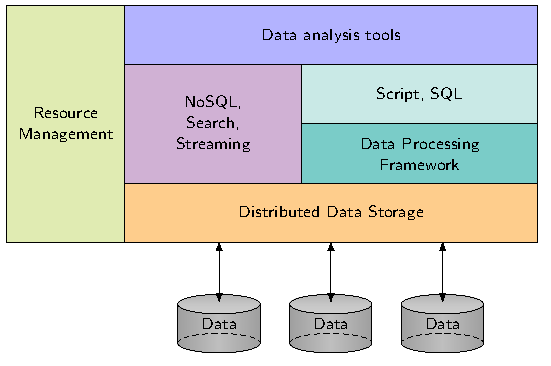
\includegraphics[width=\linewidth]{letters/Figures/big-architecture}
		\caption{Big Data Software Architecture.}
		\label{fig:bigdata}
	\end{minipage}%
	\begin{minipage}{.5\textwidth}
		\centering
		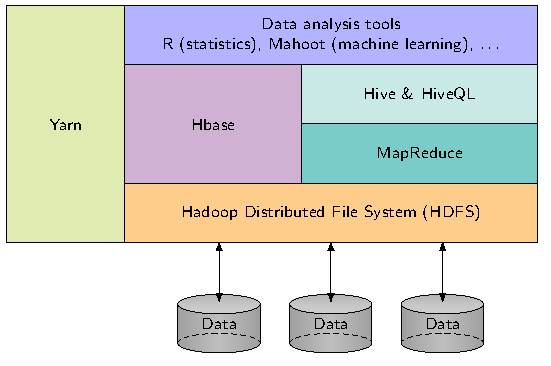
\includegraphics[width=\linewidth]{letters/Figures/Hadoop-stack}
		\caption{Current Instantiation based on MapReduce.}
		\label{fig:hadoop}
	\end{minipage}
%	\caption{A figure with two subfigures}\re
	\label{fig:test}
\end{figure}

The current realization of the software stack (or architecture) is not likely to remain dominant in the future. Components have already started to change; for example, Spark has mostly replaced Hadoop. However, it is quite likely that we will still be working with a version of the more generic architecture. How that will evolve is a matter of future research.

\section{Who Owns Data Science?}

I have avoided discussing the elephant in the room until the end -- who owns data science? Unfortunately, this has become a major issue among research communities. The argument primarily seems to be between statisticians and computer scientists, and within computer science itself; for example, between the artificial intelligence (AI) and machine learning (ML) community and others (for example, the data management community). I want to briefly present my understanding of these controversies and express my views, but my intention is not to provide an extensive analysis of different claims -- I am neither positioned nor interested in that exercise.

The concern among statisticians regarding the field of data science is long-standing. In a 2013 opinion piece in the Magazine of the American Statistical Organization, Davidian laments the absence of statisticians in a multi-institution data science initiative and asks if data science is not what statisticians do \cite{Davidian2013}. She indicates that data science is ``described as a blend of computer science, mathematics, data visualization, machine learning, distributed data management--and statistics'', almost disappointed that these disciplines are involved along with statistics. Similarly,  Donoho, in an article entitled ``50 Years of Data Science'', laments the current popular interest in data science, indicating that most statisticians view new data science programs as ``cultural appropriation''. In an extensive treatise, he argues that ``there is a solid case for some entity called `data science' to be created, which would be a true science: facing essential questions of a lasting nature and using scientifically rigorous techniques to attack those questions''. He continues: ``Insightful statisticians have for at least 50 years been laying the groundwork for constructing that would-be entity as an enlargement of traditional academic statistics. This would-be notion of data science is not the same as the data science being touted today, although there is significant overlap''\cite{Donoho2017}. There are a number of similar treatises from statisticians and the rejoinders from those who consider themselves data science researchers. Ulmann's piece \cite{Ullman:2020aa} is one of these.

Within computer science, there is a discussion regarding the relationship of AI/ML with data science. There is an obvious overlap between the two areas in the use of machine learning, and particularly deep learning, for modelling and prediction. However, it is important to note that data science and AI are distinct areas with their own research issues independent of their overlapping interest in machine learning and algorithms for analytics. Outside of this overlap, data science involves a broad set of other research topics that include data quality and trustability, big data management, interpretation and explanation of models and techniques, including visualization, as well as data security, ethics, and policy. Similarly, AI has a research agenda far broader than ML, although the latter is the subject of significant recent interest.

My personal view of these controversies is that they are not helpful; they do not move the data science agenda forward. It may help each community to feel good -- we are defending our central role in this exciting new field -- but in the long run, it is not helpful. No single community ``owns'' data science -- it is too big, the challenges are too great, and it requires involvement from many disciplines. I hope this viewpoint generates some discussion as the community collectively works to properly investigate and scope this field, perhaps turning it into a well-defined discipline.

\section{Conclusions}

Although we have been talking about data science for some years, the field is still in its infancy and there is much work that needs to be done to scope and position it properly. The success of early data science applications is evident: from health sciences, where social network analytics have enabled the tracking of epidemics; to financial systems, where guidance of investment decisions are based on the analysis of large volumes of data; to the customer care industry, where advances in speech recognition have led to the development of chatbots for customer service. However, these advances only hint at what is possible; the full impact of data science has yet to be realized. Significant improvements are required in fundamental aspects of data science and in the development of integrated processes that turn data into insight. In particular, current developments tend to be isolated to sub-fields of data science, and do not consider the entire lifecycle as I have discussed it in this article. This siloing is significantly impeding large-scale advances. As a result, the capacity for data science applications to incorporate new foundational technologies is lagging.

Furthermore, I strongly believe that we have a lot of interesting work to do in collaboration with colleagues in the social sciences and humanities. I hinted at some of these, but a full treatment of possibilities exceeds the purpose of this article. My conviction has been strengthened by my involvement in the STEM For Global Resilience research cluster in the Balsillie School of International Affairs\footnote{\url{https://www.balsillieschool.ca/research/clusters/stem/}}. The interaction of STEM researchers with those in the social sciences and humanities has potential for many exciting avenues of research.

The objective of this article is to lay out a systematic view of the data science field. The key messages are that: (1) we need to clearly establish how we view the entire field; (2) we need to take a holistic view of activities that comprise data science; and (3) we must establish a framework that facilitates cooperation and collaboration among a number of disciplines. 


\section{Acknowledgements}
Raymond Ng (CS, University of British Columbia) and Nancy Reid (Statistics, University of Toronto) were co-PIs on the original proposal to form a nation-wide centre and they contributed in a major way to the vision outlined here. Many colleagues from many institutions across Canada also contributed. The subsequent proposal to form the Waterloo Data Science Institute (DSI) was created in collaboration with a large number of colleagues (too many to list here) from every Faculty at the University of Waterloo. The vision proposed in this article can be considered a collective community effort to scope the data science field. I express my personal thanks to Brittany Reiche of the University of Waterloo. She helped develop the Waterloo Data Science Institute proposal and she helped with this opinion piece -- not only editing it, but making sure that my arguments held up.

%\bibliographystyle{abbrv}
%
%\bibliography{publishers,publications,misc,references}

\begin{thebibliography}{1}

\bibitem{Davidian2013}
M.~Davidian.
\newblock Aren't we data science?
\newblock {\em Magazine of American Statistical Association}, 2013.

\bibitem{Donoho2017}
D.~Donoho.
\newblock 50 years of data science.
\newblock {\em J. Computational and Graphical Statistics}, 26(4):745--766,
  2017.

\bibitem{Hayashi:1998aa}
C.~Hayashi.
\newblock What is data science? fundamental concepts and a heuristic example.
\newblock In C.~Hayashi, K.~Yajima, H.-H. Bock, N.~Ohsumi, Y.~Tanaka, and
  Y.~Baba, editors, {\em Data Science, Classification, and Related Methods},
  pages 40--51. Springer Japan, 1998.

\bibitem{hey2009the}
T.~Hey, S.~Tansley, and K.~Tolle.
\newblock {\em The Fourth Paradigm: Data-Intensive Scientific Discovery}.
\newblock Microsoft Research, October 2009.

\bibitem{OzsuV:2020aa}
M.~T. {\"O}zsu and P.~Valduriez.
\newblock {\em Principles of Distributed Database Systems}.
\newblock Springer, 4th edition, 2020.

\bibitem{Ullman:2020aa}
J.~D. Ullman.
\newblock The battle for data science.
\newblock {\em Q. Bull. IEEE TC on Data Eng.}, 43(2):8--14, 2020.

\end{thebibliography}

\end{document} 
